\documentclass[xcolor=svgnames,9pt,english,aspectratio=169,t]{beamer}
%\documentclass[xcolor=svgnames,9pt,english,handout,aspectratio=169,t]{beamer}
\newcommand{\handout}{0}

% =====================================================================
% POLI 450A (2026) --- shared TEMPLATE layer.
%
% Input from each lecture near the top of its file, BEFORE
% ../course_theme.tex (metropolis must be selected before the course
% palette overrides it):
%
%   \documentclass[xcolor=svgnames,9pt,english,aspectratio=169]{beamer}
%   \newcommand{\handout}{0}
%   % =====================================================================
% POLI 450A (2026) --- shared TEMPLATE layer.
%
% Input from each lecture near the top of its file, BEFORE
% ../course_theme.tex (metropolis must be selected before the course
% palette overrides it):
%
%   \documentclass[xcolor=svgnames,9pt,english,aspectratio=169]{beamer}
%   \newcommand{\handout}{0}
%   % =====================================================================
% POLI 450A (2026) --- shared TEMPLATE layer.
%
% Input from each lecture near the top of its file, BEFORE
% ../course_theme.tex (metropolis must be selected before the course
% palette overrides it):
%
%   \documentclass[xcolor=svgnames,9pt,english,aspectratio=169]{beamer}
%   \newcommand{\handout}{0}
%   \input{../course_preamble.tex}
%   \input{../course_theme.tex}
%   \graphicspath{{./}{./figs/}}
%   \title[Short title]{450A Political Methodology I}
%   \subtitle{Lecture N: ...}
%
% Modeled on the 2026 Northwestern workshop template
% (Teaching/PanelData/_latex/2026/202608_Northwestern/workshop_preamble.tex).
%
% SCOPE: theme, beamer layout, packages, the roadmap hooks, and --- unlike
% the Northwestern decks --- the notation macros. The 450A lectures
% grew from one common ancestor, so their macro blocks agree wherever they
% overlap; merging them is safe. Three points where they had drifted are
% resolved here, and each is flagged inline below.
% =====================================================================

\usetheme{metropolis}
\metroset{sectionpage=none, subsectionpage=none, numbering=none}
\setbeamertemplate{navigation symbols}{}

\setbeamersize{text margin left=5mm, text margin right=5mm}
\setbeamertemplate{itemize/enumerate body begin}{\leftmargini=1.5em\relax}
\setbeamertemplate{itemize/enumerate subbody begin}{\leftmarginii=1.5em\relax}
\setbeamertemplate{itemize/enumerate subsubbody begin}{\leftmarginiii=1.5em\relax}

% ----------------------------------------------------------- top alignment
% Every deck passes the t class option, so beamer applies the frame key
% below to every frame (explicit [plain,c] frames — title page, roadmaps —
% stay centered). Beamer's stock t key puts a rigid .2cm pad above the
% content; frames sized to this template's full-height ceilings then run
% Overfull \vbox by up to that pad. Same key as beamerbaseframe.sty, with
% one change: the pad may shrink to zero when the frame is full.
\makeatletter
\define@key{beamerframe}{t}[true]{% top
  \beamer@frametopskip=.2cm plus .5\paperheight minus .2cm\relax%
  \beamer@framebottomskip=0pt plus 1fill\relax%
  \beamer@frametopskipautobreak=\beamer@frametopskip\relax%
  \beamer@framebottomskipautobreak=\beamer@framebottomskip\relax%
}

% ------------------------------------------------- slide-top check (2026-10-11)
% A slide whose content is too tall for the frame is squeezed: the pad above
% shrinks and its content starts higher than on other slides, so a figure
% "wobbles" when the class steps from one slide to the next (Lecture 4-1,
% slides 1-2, 2026-10-11). The marker below records where each slide's
% content starts (a whatsit: it adds no space and moves nothing).
% `python3 ../check_slides.py lec<N>` then lists every slide that starts
% higher than the deck's normal position. That list must be empty.
% Recorded per slide: page, frame number, content-top y (sp), the room left
% below the title bar, and P for a plain frame (title page, roadmaps).
\providecommand\slidetop[5]{}
\AtBeginDocument{\immediate\write\@auxout{\string\providecommand\string\slidetop[5]{}}}
\def\beamer@markframetop{%
  \pdfsavepos
  \edef\beamer@marktmp{\noexpand\write\noexpand\@auxout{\string\slidetop
    {\noexpand\thepage}{\noexpand\insertframenumber}{\noexpand\the\noexpand\pdflastypos}%
    {\number\beamer@frametextheight}{\ifbeamer@plainframe P\else N\fi}}}%
  \beamer@marktmp}
\RequirePackage{etoolbox}
\patchcmd{\endbeamer@frameslide}
  {\vskip\beamer@frametopskip}
  {\vskip\beamer@frametopskip\beamer@markframetop}
  {}{\PackageWarning{course_preamble}{slide-top marker not installed}}
\makeatother

% ---------------------------------------------------------------- packages
\usepackage{xcolor}
\usepackage{colortbl}
\usepackage{amsmath}
\usepackage{amsfonts}
\usepackage{amssymb}
\usepackage{bm}
\usepackage{graphicx}
\usepackage{multirow}
\usepackage{fancyvrb}
\usepackage{listings}
\usepackage{tikz}
\usetikzlibrary{arrows.meta,positioning,decorations.pathreplacing}

% --------------------------------------------------------- figure fitting
% Default bounding box for every \includegraphics that does not override it.
% With keepaspectratio the image is scaled to fit *inside* width x height, so
% a figure can never run past the side margins or off the bottom of a slide.
% Options given at the call site override these on a per-key basis: e.g.
% [width=.6\linewidth] narrows the box but keeps the height ceiling.
% \figmaxheight is set at \begin{document}: beamer only computes the final
% \textheight once the head/foot templates are known. 0.80 is just under what a
% frame with a title and one line of text can hold (measured: 0.834\textheight);
% a frame that needs more room for text can lower it locally.
\newlength{\figmaxheight}
\AtBeginDocument{\setlength{\figmaxheight}{0.80\textheight}}
\setkeys{Gin}{width=\linewidth,height=\figmaxheight,keepaspectratio}

% -------------------------------------------------------- roadmap frames
% Identical in all lectures. A lecture that does not want the
% subsection roadmap clears it after the \input with \AtBeginSubsection[]{}.
% hideothersubsections is load-bearing, not cosmetic: lecture 4 had 13
% subsections before it was split into 4-1, 4-2 and 4-3 (2026-10-09), and a
% full contents list ran off the top and bottom of the slide. Hiding the other sections' subsections caps the list at 10 lines.
\subject{Talks}
% No back-to-back roadmaps (Yiqing, 2026-10-11): when a subsection starts right
% after its section's roadmap, with no content slide in between, its own
% roadmap would repeat the one just shown (5-1's handout showed "Two Cases"
% twice), so it is skipped. The section roadmap records the frame count; the
% subsection roadmap appears only if a content slide has come since.
\makeatletter
\def\course@secframe{-1}
\AtBeginSection[]
{
  \begin{frame}[plain,c]
    \frametitle{}
    \tableofcontents[currentsection,hideothersubsections]
    \addtocounter{framenumber}{-1}
  \end{frame}
  \xdef\course@secframe{\the\c@framenumber}
}
\AtBeginSubsection[]
{
  \ifnum\c@framenumber=\course@secframe\relax\else
  \begin{frame}[plain,c]
    \frametitle{}
    \tableofcontents[currentsection,currentsubsection,hideothersubsections]
    \addtocounter{framenumber}{-1}
  \end{frame}
  \fi
}
\makeatother

% ------------------------------------------------------ theorem environments
\newtheorem{assumption}{Assumption}
\newtheorem{iass}{Identification Assumption}
\newtheorem{ires}{Identification Result}
\newtheorem{estm}{Estimand}
\newtheorem{esti}{Estimator}
\newtheorem{question}{Question}
\newtheorem{answer}{Answer}
\newtheorem{proposition}{Proposition}

% =====================================================================
% Notation
% =====================================================================
\definecolor{dgreen}{rgb}{0,.6,0.8}

\renewcommand\r{\right}
\renewcommand\l{\left}
\newcommand{\bs}{\boldsymbol}
\newcommand{\mb}{\mathbf}
\newcommand{\real}{\mathbb{R}}
\newcommand{\cN}{\mathcal{N}}
\newcommand{\E}{\mathbb{E}}
\newcommand{\V}{\mathbb{V}}

% MERGE NOTE 1. Lecture 2-4 set \epsilon to \varepsilon; the other twelve
% left it at the upright default. Adopting \varepsilon course-wide so the
% error term looks the same in every lecture.
\renewcommand{\epsilon}{\varepsilon}

% MERGE NOTE 2. Lecture 2-4 wrote its vectors as \bm (bold italic); the other
% twelve use \mathbf (bold upright). \mathbf wins --- it is the convention in
% eleven of the thirteen decks and in the course's matrix lectures. Only
% \iid, \E, \cN and \Var from that block are actually used in 2-4's body.
\renewcommand{\u}{\ensuremath{\mb{u}}}
\renewcommand{\v}{\ensuremath{\mb{v}}}
\newcommand{\U}{\ensuremath{\mb{U}}}
\newcommand{\M}{\ensuremath{\mb{M}}}
\newcommand{\X}{\ensuremath{\mb{X}}}
\newcommand{\x}{\ensuremath{\mb{x}}}
\newcommand{\y}{\ensuremath{\mb{y}}}
\newcommand{\Z}{\ensuremath{\mb{Z}}}
\newcommand{\C}{\ensuremath{\mb{C}}}
\newcommand{\D}{\ensuremath{\mb{D}}}
\newcommand{\I}{\ensuremath{\mb{I}}}
\newcommand{\W}{\ensuremath{\mb{W}}}
\renewcommand{\a}{\ensuremath{\mb{a}}}
\renewcommand{\P}{\ensuremath{\mb{P}}}
\newcommand{\one}{\ensuremath{\mb{1}}}
\newcommand{\zero}{\ensuremath{\mb{0}}}

\renewcommand{\b}{\ensuremath{\bs{\beta}}}
\newcommand{\be}{\ensuremath{\bs{\beta}}}
\newcommand{\e}{\ensuremath{\bs{\epsilon}}}
\newcommand{\eps}{\ensuremath{\bs{\epsilon}}}
\newcommand{\eeta}{\ensuremath{\bs{\eta}}}
\newcommand{\bhat}{\ensuremath{\hat{\bs{\beta}}}}
\newcommand{\ehat}{\ensuremath{\hat{\e}}}
\newcommand{\Sig}{\ensuremath{\bs{\Sigma}}}
\newcommand{\SigInv}{\ensuremath{\bs{\Sigma^{-1}}}}

\newcommand{\XX}{\ensuremath{\X'\X}}
\newcommand{\XXinv}{\ensuremath{\left(\XX\right)^{-1}}}
\newcommand{\hatmat}{\ensuremath{\X \XXinv \X'}}
\newcommand{\hatsig}{\ensuremath{\hat{\sigma}^2}}
\newcommand{\sig}{\ensuremath{\sigma^2}}

\newcommand{\cA}{\mathcal{A}}
\newcommand{\cJ}{\mathcal{J}}
\newcommand{\cL}{\mathcal{L}}
\newcommand{\cLL}{\mathcal{LL}}
\newcommand{\cll}{\ell}
\newcommand{\cQ}{\mathcal{Q}}
\newcommand{\cP}{\mathcal{P}}

% MERGE NOTE 3. \var / \Var and \cov / \Cov were spelled with \text in some
% lectures and \mbox in others. Same output; \text kept.
\newcommand{\var}{\text{Var}}
\newcommand{\Var}{\text{Var}}
\newcommand{\cov}{\text{Cov}}
\newcommand{\Cov}{\text{Cov}}
\newcommand{\cor}{\text{Cor}}
\newcommand{\tr}{\text{tr}}
\newcommand{\avepop}{\frac{1}{n}\sum_{i=1}^n}

\DeclareMathOperator*\plim{plim}
\DeclareMathOperator\rank{rank}
\DeclareMathOperator*\argmax{argmax}
\DeclareMathOperator*\argmin{argmin}
\DeclareMathOperator{\sgn}{sgn}
\newcommand{\diag}{\mathop{\mathrm{diag}}}

\newcommand\ud{\mathrm{d}}
\newcommand\dist{\buildrel\rm d\over\sim}
\newcommand\ind{\stackrel{\rm indep.}{\sim}}
\newcommand\iid{\stackrel{\rm i.i.d.}{\sim}}
\newcommand\logit{{\rm logit}}

\newcommand\indep{\protect\mathpalette{\protect\independenT}{\perp}}
\def\independenT#1#2{\mathrel{\rlap{$#1#2$}\mkern2mu{#1#2}}}

% ------------------------------------------------------------- text helpers
\newcommand{\bi}{\begin{itemize}}
\newcommand{\ei}{\end{itemize}}
\newcommand{\noi}{\noindent}
\newcommand{\red}{\textcolor{Cardinal}}
\newcommand{\blue}{\textcolor{CourseBlue}}
\newcommand{\gray}{\textcolor{gray}}
\newcommand\spacingset[1]{\renewcommand{\baselinestretch}{#1}\small\normalsize}

\hyphenation{tyamamot}


% ------------------------------------------------ figure-position check (2026-10-11)
% Records where every \includegraphics lands and its size (a whatsit; it moves
% nothing). check_slides.py flags two consecutive slides that show a figure of
% the same size in different places: the class sees it jump (Lecture 3, slides
% 18 to 19: one frame had \vspace{.3cm} above the figure, the next did not),
% and two consecutive slides that show the same file at different sizes or
% places (Lecture 6-3, slides 10 to 11, the ballot image). The file name is the
% seventh field.
\makeatletter
\providecommand\figpos[7]{}
\AtBeginDocument{\immediate\write\@auxout{\string\providecommand\string\figpos[7]{}}}
\newbox\course@figbox
\let\course@origGinclude\Ginclude@graphics
\def\Ginclude@graphics#1{%
  \setbox\course@figbox\hbox{\course@origGinclude{#1}}%
  \pdfsavepos
  \edef\course@figtmp{\noexpand\write\noexpand\@auxout{\string\figpos
    {\noexpand\thepage}{\noexpand\insertframenumber}%
    {\noexpand\the\noexpand\pdflastxpos}{\noexpand\the\noexpand\pdflastypos}%
    {\number\wd\course@figbox}{\number\ht\course@figbox}{\detokenize{#1}}}}%
  \course@figtmp
  \box\course@figbox}
\makeatother

%   % =====================================================================
% POLI 450A (2026) --- shared visual system.
% Input from each lecture AFTER ../course_preamble.tex.
%
% Same shape as the 2026 Northwestern workshop theme
% (Teaching/PanelData/_latex/2026/202608_Northwestern/workshop_theme.tex),
% with the workshop's purple swapped for the course's cardinal. Kept
% deliberately light so the lecture sources stay easy to edit.
%
% To retune the course to Stanford's official cardinal, change the one
% Cardinal line below to HTML 8C1515.
% =====================================================================
\definecolor{Cardinal}{HTML}{A8003B}     % primary: titles, structure, alerts
\definecolor{CourseInk}{HTML}{252A34}    % body text
\definecolor{CourseBlue}{HTML}{2F6B9A}   % secondary accent
\definecolor{CourseMist}{HTML}{F8F1F4}   % block backgrounds

\setbeamercolor{normal text}{fg=CourseInk,bg=white}
\setbeamercolor{structure}{fg=Cardinal}
\setbeamercolor{alerted text}{fg=Cardinal}
\setbeamercolor{frametitle}{fg=white,bg=Cardinal}
\setbeamercolor{title}{fg=Cardinal}
\setbeamercolor{subtitle}{fg=CourseInk}
\setbeamercolor{block title}{fg=white,bg=Cardinal}
\setbeamercolor{block body}{fg=CourseInk,bg=CourseMist}
\setbeamercolor{section in toc}{fg=Cardinal}
\setbeamercolor{subsection in toc}{fg=CourseInk}
\setbeamercolor{itemize item}{fg=Cardinal}
\setbeamercolor{itemize subitem}{fg=Cardinal}
\setbeamercolor{enumerate item}{fg=Cardinal}

\setbeamerfont{title}{series=\bfseries,size=\Large}
\setbeamerfont{frametitle}{series=\bfseries,size=\large}
\setbeamerfont{block title}{series=\bfseries}
\setbeamertemplate{navigation symbols}{}
\setbeamertemplate{items}[circle]
\setbeamertemplate{blocks}[rounded][shadow=false]
\setbeamertemplate{frametitle continuation}{}
\setbeamertemplate{footline}{%
  \leavevmode\hbox{%
  \begin{beamercolorbox}[wd=.88\paperwidth,ht=2.6ex,dp=1.2ex,leftskip=1.2em]{author in head/foot}%
  \usebeamerfont{author in head/foot}\insertshorttitle
  \end{beamercolorbox}%
  \begin{beamercolorbox}[wd=.12\paperwidth,ht=2.6ex,dp=1.2ex,center]{date in head/foot}%
  \insertframenumber
  \end{beamercolorbox}}}

\newcommand{\slidesource}[1]{\vfill{\scriptsize\color{gray}Source: #1}}
\newcommand{\keyquestion}[1]{\begin{block}{Question}#1\end{block}}

%   \graphicspath{{./}{./figs/}}
%   \title[Short title]{450A Political Methodology I}
%   \subtitle{Lecture N: ...}
%
% Modeled on the 2026 Northwestern workshop template
% (Teaching/PanelData/_latex/2026/202608_Northwestern/workshop_preamble.tex).
%
% SCOPE: theme, beamer layout, packages, the roadmap hooks, and --- unlike
% the Northwestern decks --- the notation macros. The 450A lectures
% grew from one common ancestor, so their macro blocks agree wherever they
% overlap; merging them is safe. Three points where they had drifted are
% resolved here, and each is flagged inline below.
% =====================================================================

\usetheme{metropolis}
\metroset{sectionpage=none, subsectionpage=none, numbering=none}
\setbeamertemplate{navigation symbols}{}

\setbeamersize{text margin left=5mm, text margin right=5mm}
\setbeamertemplate{itemize/enumerate body begin}{\leftmargini=1.5em\relax}
\setbeamertemplate{itemize/enumerate subbody begin}{\leftmarginii=1.5em\relax}
\setbeamertemplate{itemize/enumerate subsubbody begin}{\leftmarginiii=1.5em\relax}

% ----------------------------------------------------------- top alignment
% Every deck passes the t class option, so beamer applies the frame key
% below to every frame (explicit [plain,c] frames — title page, roadmaps —
% stay centered). Beamer's stock t key puts a rigid .2cm pad above the
% content; frames sized to this template's full-height ceilings then run
% Overfull \vbox by up to that pad. Same key as beamerbaseframe.sty, with
% one change: the pad may shrink to zero when the frame is full.
\makeatletter
\define@key{beamerframe}{t}[true]{% top
  \beamer@frametopskip=.2cm plus .5\paperheight minus .2cm\relax%
  \beamer@framebottomskip=0pt plus 1fill\relax%
  \beamer@frametopskipautobreak=\beamer@frametopskip\relax%
  \beamer@framebottomskipautobreak=\beamer@framebottomskip\relax%
}

% ------------------------------------------------- slide-top check (2026-10-11)
% A slide whose content is too tall for the frame is squeezed: the pad above
% shrinks and its content starts higher than on other slides, so a figure
% "wobbles" when the class steps from one slide to the next (Lecture 4-1,
% slides 1-2, 2026-10-11). The marker below records where each slide's
% content starts (a whatsit: it adds no space and moves nothing).
% `python3 ../check_slides.py lec<N>` then lists every slide that starts
% higher than the deck's normal position. That list must be empty.
% Recorded per slide: page, frame number, content-top y (sp), the room left
% below the title bar, and P for a plain frame (title page, roadmaps).
\providecommand\slidetop[5]{}
\AtBeginDocument{\immediate\write\@auxout{\string\providecommand\string\slidetop[5]{}}}
\def\beamer@markframetop{%
  \pdfsavepos
  \edef\beamer@marktmp{\noexpand\write\noexpand\@auxout{\string\slidetop
    {\noexpand\thepage}{\noexpand\insertframenumber}{\noexpand\the\noexpand\pdflastypos}%
    {\number\beamer@frametextheight}{\ifbeamer@plainframe P\else N\fi}}}%
  \beamer@marktmp}
\RequirePackage{etoolbox}
\patchcmd{\endbeamer@frameslide}
  {\vskip\beamer@frametopskip}
  {\vskip\beamer@frametopskip\beamer@markframetop}
  {}{\PackageWarning{course_preamble}{slide-top marker not installed}}
\makeatother

% ---------------------------------------------------------------- packages
\usepackage{xcolor}
\usepackage{colortbl}
\usepackage{amsmath}
\usepackage{amsfonts}
\usepackage{amssymb}
\usepackage{bm}
\usepackage{graphicx}
\usepackage{multirow}
\usepackage{fancyvrb}
\usepackage{listings}
\usepackage{tikz}
\usetikzlibrary{arrows.meta,positioning,decorations.pathreplacing}

% --------------------------------------------------------- figure fitting
% Default bounding box for every \includegraphics that does not override it.
% With keepaspectratio the image is scaled to fit *inside* width x height, so
% a figure can never run past the side margins or off the bottom of a slide.
% Options given at the call site override these on a per-key basis: e.g.
% [width=.6\linewidth] narrows the box but keeps the height ceiling.
% \figmaxheight is set at \begin{document}: beamer only computes the final
% \textheight once the head/foot templates are known. 0.80 is just under what a
% frame with a title and one line of text can hold (measured: 0.834\textheight);
% a frame that needs more room for text can lower it locally.
\newlength{\figmaxheight}
\AtBeginDocument{\setlength{\figmaxheight}{0.80\textheight}}
\setkeys{Gin}{width=\linewidth,height=\figmaxheight,keepaspectratio}

% -------------------------------------------------------- roadmap frames
% Identical in all lectures. A lecture that does not want the
% subsection roadmap clears it after the \input with \AtBeginSubsection[]{}.
% hideothersubsections is load-bearing, not cosmetic: lecture 4 had 13
% subsections before it was split into 4-1, 4-2 and 4-3 (2026-10-09), and a
% full contents list ran off the top and bottom of the slide. Hiding the other sections' subsections caps the list at 10 lines.
\subject{Talks}
% No back-to-back roadmaps (Yiqing, 2026-10-11): when a subsection starts right
% after its section's roadmap, with no content slide in between, its own
% roadmap would repeat the one just shown (5-1's handout showed "Two Cases"
% twice), so it is skipped. The section roadmap records the frame count; the
% subsection roadmap appears only if a content slide has come since.
\makeatletter
\def\course@secframe{-1}
\AtBeginSection[]
{
  \begin{frame}[plain,c]
    \frametitle{}
    \tableofcontents[currentsection,hideothersubsections]
    \addtocounter{framenumber}{-1}
  \end{frame}
  \xdef\course@secframe{\the\c@framenumber}
}
\AtBeginSubsection[]
{
  \ifnum\c@framenumber=\course@secframe\relax\else
  \begin{frame}[plain,c]
    \frametitle{}
    \tableofcontents[currentsection,currentsubsection,hideothersubsections]
    \addtocounter{framenumber}{-1}
  \end{frame}
  \fi
}
\makeatother

% ------------------------------------------------------ theorem environments
\newtheorem{assumption}{Assumption}
\newtheorem{iass}{Identification Assumption}
\newtheorem{ires}{Identification Result}
\newtheorem{estm}{Estimand}
\newtheorem{esti}{Estimator}
\newtheorem{question}{Question}
\newtheorem{answer}{Answer}
\newtheorem{proposition}{Proposition}

% =====================================================================
% Notation
% =====================================================================
\definecolor{dgreen}{rgb}{0,.6,0.8}

\renewcommand\r{\right}
\renewcommand\l{\left}
\newcommand{\bs}{\boldsymbol}
\newcommand{\mb}{\mathbf}
\newcommand{\real}{\mathbb{R}}
\newcommand{\cN}{\mathcal{N}}
\newcommand{\E}{\mathbb{E}}
\newcommand{\V}{\mathbb{V}}

% MERGE NOTE 1. Lecture 2-4 set \epsilon to \varepsilon; the other twelve
% left it at the upright default. Adopting \varepsilon course-wide so the
% error term looks the same in every lecture.
\renewcommand{\epsilon}{\varepsilon}

% MERGE NOTE 2. Lecture 2-4 wrote its vectors as \bm (bold italic); the other
% twelve use \mathbf (bold upright). \mathbf wins --- it is the convention in
% eleven of the thirteen decks and in the course's matrix lectures. Only
% \iid, \E, \cN and \Var from that block are actually used in 2-4's body.
\renewcommand{\u}{\ensuremath{\mb{u}}}
\renewcommand{\v}{\ensuremath{\mb{v}}}
\newcommand{\U}{\ensuremath{\mb{U}}}
\newcommand{\M}{\ensuremath{\mb{M}}}
\newcommand{\X}{\ensuremath{\mb{X}}}
\newcommand{\x}{\ensuremath{\mb{x}}}
\newcommand{\y}{\ensuremath{\mb{y}}}
\newcommand{\Z}{\ensuremath{\mb{Z}}}
\newcommand{\C}{\ensuremath{\mb{C}}}
\newcommand{\D}{\ensuremath{\mb{D}}}
\newcommand{\I}{\ensuremath{\mb{I}}}
\newcommand{\W}{\ensuremath{\mb{W}}}
\renewcommand{\a}{\ensuremath{\mb{a}}}
\renewcommand{\P}{\ensuremath{\mb{P}}}
\newcommand{\one}{\ensuremath{\mb{1}}}
\newcommand{\zero}{\ensuremath{\mb{0}}}

\renewcommand{\b}{\ensuremath{\bs{\beta}}}
\newcommand{\be}{\ensuremath{\bs{\beta}}}
\newcommand{\e}{\ensuremath{\bs{\epsilon}}}
\newcommand{\eps}{\ensuremath{\bs{\epsilon}}}
\newcommand{\eeta}{\ensuremath{\bs{\eta}}}
\newcommand{\bhat}{\ensuremath{\hat{\bs{\beta}}}}
\newcommand{\ehat}{\ensuremath{\hat{\e}}}
\newcommand{\Sig}{\ensuremath{\bs{\Sigma}}}
\newcommand{\SigInv}{\ensuremath{\bs{\Sigma^{-1}}}}

\newcommand{\XX}{\ensuremath{\X'\X}}
\newcommand{\XXinv}{\ensuremath{\left(\XX\right)^{-1}}}
\newcommand{\hatmat}{\ensuremath{\X \XXinv \X'}}
\newcommand{\hatsig}{\ensuremath{\hat{\sigma}^2}}
\newcommand{\sig}{\ensuremath{\sigma^2}}

\newcommand{\cA}{\mathcal{A}}
\newcommand{\cJ}{\mathcal{J}}
\newcommand{\cL}{\mathcal{L}}
\newcommand{\cLL}{\mathcal{LL}}
\newcommand{\cll}{\ell}
\newcommand{\cQ}{\mathcal{Q}}
\newcommand{\cP}{\mathcal{P}}

% MERGE NOTE 3. \var / \Var and \cov / \Cov were spelled with \text in some
% lectures and \mbox in others. Same output; \text kept.
\newcommand{\var}{\text{Var}}
\newcommand{\Var}{\text{Var}}
\newcommand{\cov}{\text{Cov}}
\newcommand{\Cov}{\text{Cov}}
\newcommand{\cor}{\text{Cor}}
\newcommand{\tr}{\text{tr}}
\newcommand{\avepop}{\frac{1}{n}\sum_{i=1}^n}

\DeclareMathOperator*\plim{plim}
\DeclareMathOperator\rank{rank}
\DeclareMathOperator*\argmax{argmax}
\DeclareMathOperator*\argmin{argmin}
\DeclareMathOperator{\sgn}{sgn}
\newcommand{\diag}{\mathop{\mathrm{diag}}}

\newcommand\ud{\mathrm{d}}
\newcommand\dist{\buildrel\rm d\over\sim}
\newcommand\ind{\stackrel{\rm indep.}{\sim}}
\newcommand\iid{\stackrel{\rm i.i.d.}{\sim}}
\newcommand\logit{{\rm logit}}

\newcommand\indep{\protect\mathpalette{\protect\independenT}{\perp}}
\def\independenT#1#2{\mathrel{\rlap{$#1#2$}\mkern2mu{#1#2}}}

% ------------------------------------------------------------- text helpers
\newcommand{\bi}{\begin{itemize}}
\newcommand{\ei}{\end{itemize}}
\newcommand{\noi}{\noindent}
\newcommand{\red}{\textcolor{Cardinal}}
\newcommand{\blue}{\textcolor{CourseBlue}}
\newcommand{\gray}{\textcolor{gray}}
\newcommand\spacingset[1]{\renewcommand{\baselinestretch}{#1}\small\normalsize}

\hyphenation{tyamamot}


% ------------------------------------------------ figure-position check (2026-10-11)
% Records where every \includegraphics lands and its size (a whatsit; it moves
% nothing). check_slides.py flags two consecutive slides that show a figure of
% the same size in different places: the class sees it jump (Lecture 3, slides
% 18 to 19: one frame had \vspace{.3cm} above the figure, the next did not),
% and two consecutive slides that show the same file at different sizes or
% places (Lecture 6-3, slides 10 to 11, the ballot image). The file name is the
% seventh field.
\makeatletter
\providecommand\figpos[7]{}
\AtBeginDocument{\immediate\write\@auxout{\string\providecommand\string\figpos[7]{}}}
\newbox\course@figbox
\let\course@origGinclude\Ginclude@graphics
\def\Ginclude@graphics#1{%
  \setbox\course@figbox\hbox{\course@origGinclude{#1}}%
  \pdfsavepos
  \edef\course@figtmp{\noexpand\write\noexpand\@auxout{\string\figpos
    {\noexpand\thepage}{\noexpand\insertframenumber}%
    {\noexpand\the\noexpand\pdflastxpos}{\noexpand\the\noexpand\pdflastypos}%
    {\number\wd\course@figbox}{\number\ht\course@figbox}{\detokenize{#1}}}}%
  \course@figtmp
  \box\course@figbox}
\makeatother

%   % =====================================================================
% POLI 450A (2026) --- shared visual system.
% Input from each lecture AFTER ../course_preamble.tex.
%
% Same shape as the 2026 Northwestern workshop theme
% (Teaching/PanelData/_latex/2026/202608_Northwestern/workshop_theme.tex),
% with the workshop's purple swapped for the course's cardinal. Kept
% deliberately light so the lecture sources stay easy to edit.
%
% To retune the course to Stanford's official cardinal, change the one
% Cardinal line below to HTML 8C1515.
% =====================================================================
\definecolor{Cardinal}{HTML}{A8003B}     % primary: titles, structure, alerts
\definecolor{CourseInk}{HTML}{252A34}    % body text
\definecolor{CourseBlue}{HTML}{2F6B9A}   % secondary accent
\definecolor{CourseMist}{HTML}{F8F1F4}   % block backgrounds

\setbeamercolor{normal text}{fg=CourseInk,bg=white}
\setbeamercolor{structure}{fg=Cardinal}
\setbeamercolor{alerted text}{fg=Cardinal}
\setbeamercolor{frametitle}{fg=white,bg=Cardinal}
\setbeamercolor{title}{fg=Cardinal}
\setbeamercolor{subtitle}{fg=CourseInk}
\setbeamercolor{block title}{fg=white,bg=Cardinal}
\setbeamercolor{block body}{fg=CourseInk,bg=CourseMist}
\setbeamercolor{section in toc}{fg=Cardinal}
\setbeamercolor{subsection in toc}{fg=CourseInk}
\setbeamercolor{itemize item}{fg=Cardinal}
\setbeamercolor{itemize subitem}{fg=Cardinal}
\setbeamercolor{enumerate item}{fg=Cardinal}

\setbeamerfont{title}{series=\bfseries,size=\Large}
\setbeamerfont{frametitle}{series=\bfseries,size=\large}
\setbeamerfont{block title}{series=\bfseries}
\setbeamertemplate{navigation symbols}{}
\setbeamertemplate{items}[circle]
\setbeamertemplate{blocks}[rounded][shadow=false]
\setbeamertemplate{frametitle continuation}{}
\setbeamertemplate{footline}{%
  \leavevmode\hbox{%
  \begin{beamercolorbox}[wd=.88\paperwidth,ht=2.6ex,dp=1.2ex,leftskip=1.2em]{author in head/foot}%
  \usebeamerfont{author in head/foot}\insertshorttitle
  \end{beamercolorbox}%
  \begin{beamercolorbox}[wd=.12\paperwidth,ht=2.6ex,dp=1.2ex,center]{date in head/foot}%
  \insertframenumber
  \end{beamercolorbox}}}

\newcommand{\slidesource}[1]{\vfill{\scriptsize\color{gray}Source: #1}}
\newcommand{\keyquestion}[1]{\begin{block}{Question}#1\end{block}}

%   \graphicspath{{./}{./figs/}}
%   \title[Short title]{450A Political Methodology I}
%   \subtitle{Lecture N: ...}
%
% Modeled on the 2026 Northwestern workshop template
% (Teaching/PanelData/_latex/2026/202608_Northwestern/workshop_preamble.tex).
%
% SCOPE: theme, beamer layout, packages, the roadmap hooks, and --- unlike
% the Northwestern decks --- the notation macros. The 450A lectures
% grew from one common ancestor, so their macro blocks agree wherever they
% overlap; merging them is safe. Three points where they had drifted are
% resolved here, and each is flagged inline below.
% =====================================================================

\usetheme{metropolis}
\metroset{sectionpage=none, subsectionpage=none, numbering=none}
\setbeamertemplate{navigation symbols}{}

\setbeamersize{text margin left=5mm, text margin right=5mm}
\setbeamertemplate{itemize/enumerate body begin}{\leftmargini=1.5em\relax}
\setbeamertemplate{itemize/enumerate subbody begin}{\leftmarginii=1.5em\relax}
\setbeamertemplate{itemize/enumerate subsubbody begin}{\leftmarginiii=1.5em\relax}

% ----------------------------------------------------------- top alignment
% Every deck passes the t class option, so beamer applies the frame key
% below to every frame (explicit [plain,c] frames — title page, roadmaps —
% stay centered). Beamer's stock t key puts a rigid .2cm pad above the
% content; frames sized to this template's full-height ceilings then run
% Overfull \vbox by up to that pad. Same key as beamerbaseframe.sty, with
% one change: the pad may shrink to zero when the frame is full.
\makeatletter
\define@key{beamerframe}{t}[true]{% top
  \beamer@frametopskip=.2cm plus .5\paperheight minus .2cm\relax%
  \beamer@framebottomskip=0pt plus 1fill\relax%
  \beamer@frametopskipautobreak=\beamer@frametopskip\relax%
  \beamer@framebottomskipautobreak=\beamer@framebottomskip\relax%
}

% ------------------------------------------------- slide-top check (2026-10-11)
% A slide whose content is too tall for the frame is squeezed: the pad above
% shrinks and its content starts higher than on other slides, so a figure
% "wobbles" when the class steps from one slide to the next (Lecture 4-1,
% slides 1-2, 2026-10-11). The marker below records where each slide's
% content starts (a whatsit: it adds no space and moves nothing).
% `python3 ../check_slides.py lec<N>` then lists every slide that starts
% higher than the deck's normal position. That list must be empty.
% Recorded per slide: page, frame number, content-top y (sp), the room left
% below the title bar, and P for a plain frame (title page, roadmaps).
\providecommand\slidetop[5]{}
\AtBeginDocument{\immediate\write\@auxout{\string\providecommand\string\slidetop[5]{}}}
\def\beamer@markframetop{%
  \pdfsavepos
  \edef\beamer@marktmp{\noexpand\write\noexpand\@auxout{\string\slidetop
    {\noexpand\thepage}{\noexpand\insertframenumber}{\noexpand\the\noexpand\pdflastypos}%
    {\number\beamer@frametextheight}{\ifbeamer@plainframe P\else N\fi}}}%
  \beamer@marktmp}
\RequirePackage{etoolbox}
\patchcmd{\endbeamer@frameslide}
  {\vskip\beamer@frametopskip}
  {\vskip\beamer@frametopskip\beamer@markframetop}
  {}{\PackageWarning{course_preamble}{slide-top marker not installed}}
\makeatother

% ---------------------------------------------------------------- packages
\usepackage{xcolor}
\usepackage{colortbl}
\usepackage{amsmath}
\usepackage{amsfonts}
\usepackage{amssymb}
\usepackage{bm}
\usepackage{graphicx}
\usepackage{multirow}
\usepackage{fancyvrb}
\usepackage{listings}
\usepackage{tikz}
\usetikzlibrary{arrows.meta,positioning,decorations.pathreplacing}

% --------------------------------------------------------- figure fitting
% Default bounding box for every \includegraphics that does not override it.
% With keepaspectratio the image is scaled to fit *inside* width x height, so
% a figure can never run past the side margins or off the bottom of a slide.
% Options given at the call site override these on a per-key basis: e.g.
% [width=.6\linewidth] narrows the box but keeps the height ceiling.
% \figmaxheight is set at \begin{document}: beamer only computes the final
% \textheight once the head/foot templates are known. 0.80 is just under what a
% frame with a title and one line of text can hold (measured: 0.834\textheight);
% a frame that needs more room for text can lower it locally.
\newlength{\figmaxheight}
\AtBeginDocument{\setlength{\figmaxheight}{0.80\textheight}}
\setkeys{Gin}{width=\linewidth,height=\figmaxheight,keepaspectratio}

% -------------------------------------------------------- roadmap frames
% Identical in all lectures. A lecture that does not want the
% subsection roadmap clears it after the \input with \AtBeginSubsection[]{}.
% hideothersubsections is load-bearing, not cosmetic: lecture 4 had 13
% subsections before it was split into 4-1, 4-2 and 4-3 (2026-10-09), and a
% full contents list ran off the top and bottom of the slide. Hiding the other sections' subsections caps the list at 10 lines.
\subject{Talks}
% No back-to-back roadmaps (Yiqing, 2026-10-11): when a subsection starts right
% after its section's roadmap, with no content slide in between, its own
% roadmap would repeat the one just shown (5-1's handout showed "Two Cases"
% twice), so it is skipped. The section roadmap records the frame count; the
% subsection roadmap appears only if a content slide has come since.
\makeatletter
\def\course@secframe{-1}
\AtBeginSection[]
{
  \begin{frame}[plain,c]
    \frametitle{}
    \tableofcontents[currentsection,hideothersubsections]
    \addtocounter{framenumber}{-1}
  \end{frame}
  \xdef\course@secframe{\the\c@framenumber}
}
\AtBeginSubsection[]
{
  \ifnum\c@framenumber=\course@secframe\relax\else
  \begin{frame}[plain,c]
    \frametitle{}
    \tableofcontents[currentsection,currentsubsection,hideothersubsections]
    \addtocounter{framenumber}{-1}
  \end{frame}
  \fi
}
\makeatother

% ------------------------------------------------------ theorem environments
\newtheorem{assumption}{Assumption}
\newtheorem{iass}{Identification Assumption}
\newtheorem{ires}{Identification Result}
\newtheorem{estm}{Estimand}
\newtheorem{esti}{Estimator}
\newtheorem{question}{Question}
\newtheorem{answer}{Answer}
\newtheorem{proposition}{Proposition}

% =====================================================================
% Notation
% =====================================================================
\definecolor{dgreen}{rgb}{0,.6,0.8}

\renewcommand\r{\right}
\renewcommand\l{\left}
\newcommand{\bs}{\boldsymbol}
\newcommand{\mb}{\mathbf}
\newcommand{\real}{\mathbb{R}}
\newcommand{\cN}{\mathcal{N}}
\newcommand{\E}{\mathbb{E}}
\newcommand{\V}{\mathbb{V}}

% MERGE NOTE 1. Lecture 2-4 set \epsilon to \varepsilon; the other twelve
% left it at the upright default. Adopting \varepsilon course-wide so the
% error term looks the same in every lecture.
\renewcommand{\epsilon}{\varepsilon}

% MERGE NOTE 2. Lecture 2-4 wrote its vectors as \bm (bold italic); the other
% twelve use \mathbf (bold upright). \mathbf wins --- it is the convention in
% eleven of the thirteen decks and in the course's matrix lectures. Only
% \iid, \E, \cN and \Var from that block are actually used in 2-4's body.
\renewcommand{\u}{\ensuremath{\mb{u}}}
\renewcommand{\v}{\ensuremath{\mb{v}}}
\newcommand{\U}{\ensuremath{\mb{U}}}
\newcommand{\M}{\ensuremath{\mb{M}}}
\newcommand{\X}{\ensuremath{\mb{X}}}
\newcommand{\x}{\ensuremath{\mb{x}}}
\newcommand{\y}{\ensuremath{\mb{y}}}
\newcommand{\Z}{\ensuremath{\mb{Z}}}
\newcommand{\C}{\ensuremath{\mb{C}}}
\newcommand{\D}{\ensuremath{\mb{D}}}
\newcommand{\I}{\ensuremath{\mb{I}}}
\newcommand{\W}{\ensuremath{\mb{W}}}
\renewcommand{\a}{\ensuremath{\mb{a}}}
\renewcommand{\P}{\ensuremath{\mb{P}}}
\newcommand{\one}{\ensuremath{\mb{1}}}
\newcommand{\zero}{\ensuremath{\mb{0}}}

\renewcommand{\b}{\ensuremath{\bs{\beta}}}
\newcommand{\be}{\ensuremath{\bs{\beta}}}
\newcommand{\e}{\ensuremath{\bs{\epsilon}}}
\newcommand{\eps}{\ensuremath{\bs{\epsilon}}}
\newcommand{\eeta}{\ensuremath{\bs{\eta}}}
\newcommand{\bhat}{\ensuremath{\hat{\bs{\beta}}}}
\newcommand{\ehat}{\ensuremath{\hat{\e}}}
\newcommand{\Sig}{\ensuremath{\bs{\Sigma}}}
\newcommand{\SigInv}{\ensuremath{\bs{\Sigma^{-1}}}}

\newcommand{\XX}{\ensuremath{\X'\X}}
\newcommand{\XXinv}{\ensuremath{\left(\XX\right)^{-1}}}
\newcommand{\hatmat}{\ensuremath{\X \XXinv \X'}}
\newcommand{\hatsig}{\ensuremath{\hat{\sigma}^2}}
\newcommand{\sig}{\ensuremath{\sigma^2}}

\newcommand{\cA}{\mathcal{A}}
\newcommand{\cJ}{\mathcal{J}}
\newcommand{\cL}{\mathcal{L}}
\newcommand{\cLL}{\mathcal{LL}}
\newcommand{\cll}{\ell}
\newcommand{\cQ}{\mathcal{Q}}
\newcommand{\cP}{\mathcal{P}}

% MERGE NOTE 3. \var / \Var and \cov / \Cov were spelled with \text in some
% lectures and \mbox in others. Same output; \text kept.
\newcommand{\var}{\text{Var}}
\newcommand{\Var}{\text{Var}}
\newcommand{\cov}{\text{Cov}}
\newcommand{\Cov}{\text{Cov}}
\newcommand{\cor}{\text{Cor}}
\newcommand{\tr}{\text{tr}}
\newcommand{\avepop}{\frac{1}{n}\sum_{i=1}^n}

\DeclareMathOperator*\plim{plim}
\DeclareMathOperator\rank{rank}
\DeclareMathOperator*\argmax{argmax}
\DeclareMathOperator*\argmin{argmin}
\DeclareMathOperator{\sgn}{sgn}
\newcommand{\diag}{\mathop{\mathrm{diag}}}

\newcommand\ud{\mathrm{d}}
\newcommand\dist{\buildrel\rm d\over\sim}
\newcommand\ind{\stackrel{\rm indep.}{\sim}}
\newcommand\iid{\stackrel{\rm i.i.d.}{\sim}}
\newcommand\logit{{\rm logit}}

\newcommand\indep{\protect\mathpalette{\protect\independenT}{\perp}}
\def\independenT#1#2{\mathrel{\rlap{$#1#2$}\mkern2mu{#1#2}}}

% ------------------------------------------------------------- text helpers
\newcommand{\bi}{\begin{itemize}}
\newcommand{\ei}{\end{itemize}}
\newcommand{\noi}{\noindent}
\newcommand{\red}{\textcolor{Cardinal}}
\newcommand{\blue}{\textcolor{CourseBlue}}
\newcommand{\gray}{\textcolor{gray}}
\newcommand\spacingset[1]{\renewcommand{\baselinestretch}{#1}\small\normalsize}

\hyphenation{tyamamot}


% ------------------------------------------------ figure-position check (2026-10-11)
% Records where every \includegraphics lands and its size (a whatsit; it moves
% nothing). check_slides.py flags two consecutive slides that show a figure of
% the same size in different places: the class sees it jump (Lecture 3, slides
% 18 to 19: one frame had \vspace{.3cm} above the figure, the next did not),
% and two consecutive slides that show the same file at different sizes or
% places (Lecture 6-3, slides 10 to 11, the ballot image). The file name is the
% seventh field.
\makeatletter
\providecommand\figpos[7]{}
\AtBeginDocument{\immediate\write\@auxout{\string\providecommand\string\figpos[7]{}}}
\newbox\course@figbox
\let\course@origGinclude\Ginclude@graphics
\def\Ginclude@graphics#1{%
  \setbox\course@figbox\hbox{\course@origGinclude{#1}}%
  \pdfsavepos
  \edef\course@figtmp{\noexpand\write\noexpand\@auxout{\string\figpos
    {\noexpand\thepage}{\noexpand\insertframenumber}%
    {\noexpand\the\noexpand\pdflastxpos}{\noexpand\the\noexpand\pdflastypos}%
    {\number\wd\course@figbox}{\number\ht\course@figbox}{\detokenize{#1}}}}%
  \course@figtmp
  \box\course@figbox}
\makeatother
   % theme, layout, packages, notation
% =====================================================================
% POLI 450A (2026) --- shared visual system.
% Input from each lecture AFTER ../course_preamble.tex.
%
% Same shape as the 2026 Northwestern workshop theme
% (Teaching/PanelData/_latex/2026/202608_Northwestern/workshop_theme.tex),
% with the workshop's purple swapped for the course's cardinal. Kept
% deliberately light so the lecture sources stay easy to edit.
%
% To retune the course to Stanford's official cardinal, change the one
% Cardinal line below to HTML 8C1515.
% =====================================================================
\definecolor{Cardinal}{HTML}{A8003B}     % primary: titles, structure, alerts
\definecolor{CourseInk}{HTML}{252A34}    % body text
\definecolor{CourseBlue}{HTML}{2F6B9A}   % secondary accent
\definecolor{CourseMist}{HTML}{F8F1F4}   % block backgrounds

\setbeamercolor{normal text}{fg=CourseInk,bg=white}
\setbeamercolor{structure}{fg=Cardinal}
\setbeamercolor{alerted text}{fg=Cardinal}
\setbeamercolor{frametitle}{fg=white,bg=Cardinal}
\setbeamercolor{title}{fg=Cardinal}
\setbeamercolor{subtitle}{fg=CourseInk}
\setbeamercolor{block title}{fg=white,bg=Cardinal}
\setbeamercolor{block body}{fg=CourseInk,bg=CourseMist}
\setbeamercolor{section in toc}{fg=Cardinal}
\setbeamercolor{subsection in toc}{fg=CourseInk}
\setbeamercolor{itemize item}{fg=Cardinal}
\setbeamercolor{itemize subitem}{fg=Cardinal}
\setbeamercolor{enumerate item}{fg=Cardinal}

\setbeamerfont{title}{series=\bfseries,size=\Large}
\setbeamerfont{frametitle}{series=\bfseries,size=\large}
\setbeamerfont{block title}{series=\bfseries}
\setbeamertemplate{navigation symbols}{}
\setbeamertemplate{items}[circle]
\setbeamertemplate{blocks}[rounded][shadow=false]
\setbeamertemplate{frametitle continuation}{}
\setbeamertemplate{footline}{%
  \leavevmode\hbox{%
  \begin{beamercolorbox}[wd=.88\paperwidth,ht=2.6ex,dp=1.2ex,leftskip=1.2em]{author in head/foot}%
  \usebeamerfont{author in head/foot}\insertshorttitle
  \end{beamercolorbox}%
  \begin{beamercolorbox}[wd=.12\paperwidth,ht=2.6ex,dp=1.2ex,center]{date in head/foot}%
  \insertframenumber
  \end{beamercolorbox}}}

\newcommand{\slidesource}[1]{\vfill{\scriptsize\color{gray}Source: #1}}
\newcommand{\keyquestion}[1]{\begin{block}{Question}#1\end{block}}
      % colors and slide furniture

\graphicspath{{./figs/}}

% --- Deck-local macros (added 2026-09-17) ----------------------------------
% "Hierarchy of OLS Assumptions" diagram, redrawn in TikZ from the 2012
% PowerPoint figure assumptionsfig-simple.pdf (in ../_backup/04SimpleLinearRegression_unsplit-2026-10-09/_old/figs/), with the
% same boxes and labels. Copied from deck 05-2 (lec5_2.tex) so both decks
% look alike; the only change is the first assumption (Variation in X).
% TikZ is loaded by course_preamble.tex.
% \olshierarchy{c}: c = column to emphasize (1--4); 0 draws every column in cardinal.
\newcommand{\olsitem}[1]{\ifcase#1\or Variation in $X$\or Random Sampling\or
  Linearity in Parameters\or Zero Conditional Mean\or Homoskedasticity\or
  Normality of Errors\fi}
\newcommand{\olssetcolor}[2]{%
  \ifnum#1=0 \colorlet{olsc}{Cardinal}\colorlet{olst}{CourseInk}%
  \else\ifnum#1=#2 \colorlet{olsc}{Cardinal}\colorlet{olst}{CourseInk}%
  \else \colorlet{olsc}{black!45}\colorlet{olst}{black!45}\fi\fi}
\newcommand{\olscol}[3]{% x position, header text, number of assumptions
  \node[olshd] (h) at (#1,0) {#2};
  \draw[olsln] (#1+5,-40) -- (#1+5,{-56.5-23*(#3-1)});
  \foreach \k in {1,...,#3}{%
    \node[olsit] (i) at (#1+12,{-56.5-23*(\k-1)}) {\olsitem{\k}};
    \draw[olsln] (#1+5,{-56.5-23*(\k-1)}) -- (i.west);
  }}
\newcommand{\olshierarchy}[1]{%
\begin{tikzpicture}[x=1pt,y=1pt,
    olshd/.style={anchor=north west, rounded corners=2pt, fill=olsc, text=white,
      font=\footnotesize\bfseries, align=center, text width=92pt,
      minimum height=40pt, inner sep=2pt},
    olsit/.style={anchor=west, rounded corners=2pt, draw=olsc, line width=0.6pt,
      fill=white, text=olst, font=\footnotesize, align=center, text width=84pt,
      minimum height=17pt, inner sep=2pt},
    olsln/.style={draw=olsc, line width=0.8pt}]
  \olssetcolor{#1}{1}\olscol{0}{Identification\\Data Description}{1}
  \olssetcolor{#1}{2}\olscol{106}{Unbiasedness\\Consistency}{4}
  \olssetcolor{#1}{3}\olscol{212}{Gauss--Markov (BLUE)\\Asymptotic Inference\\($z$ and $\chi^2$)}{5}
  \olssetcolor{#1}{4}\olscol{318}{Classical LM (BUE)\\Small-Sample Inference\\($t$ and $F$)}{6}
\end{tikzpicture}}
% ---------------------------------------------------------------------------

\title[Simple Regression]{450A Political Methodology I}
\subtitle{Lecture 4: Simple Regression \\ 2. Statistical Properties of Ordinary Least Squares}
\author{Stanford University}
\date{}

\begin{document}
\begin{frame}[plain,c]
  \titlepage
  \addtocounter{framenumber}{-1}
\end{frame}


\section{Statistical Properties of Ordinary Least Squares}
\frame{
\frametitle{OLS: Data Summary vs. Statistical Inference}

\begin{itemize}
\item So far (Lecture 4-1), we have studied the mechanics of OLS: how the estimates are computed from one sample.
\item That treats regression as a \alert{data summary} of the sample at hand.
\pause
\bigskip
\item However, our primary interest is to estimate $E[Y|X]$, the conditional mean/expectation function.
\item That is, we want to see linear regression as a tool for \alert{statistical inference}.
\pause
\bigskip
\item We now therefore turn to:
\begin{itemize}
  \item Treating the sample as one draw from a population model, and asking how $(\hat\beta_0,\hat\beta_1)$ behave across repeated samples
  \item A common set of assumptions for the linear regression model
  \item Properties of the OLS estimator under those assumptions
  \item Standard errors (testing, p-values, and confidence intervals follow in Lecture 4-3)
\end{itemize}
\end{itemize}
}


\frame{
\frametitle{OLS Terminology}
\small
The \alert{population} model is given by:
$$
Y = \beta_0 + \beta_1 X + u
$$
\vspace{-.22in}
\begin{itemize}
  \item $Y$: Dependent variable (outcome)
  \item $X$: Independent variable (regressor)
  \item $\beta_0$, $\beta_1$: Intercept and slope
 \item $u$: \alert{Error term} or \alert{disturbance term} \\
    --- a random variable that captures all (unobserved) factors
       which influence $Y$ other than the regressor $X$.
\end{itemize}
\pause
\bigskip
The \alert{estimated} model:
$$
Y = \hat\beta_0 + \hat\beta_1 X + \hat u
$$
\vspace{-.22in}
\begin{itemize}
  \item $\hat\beta_0$, $\hat\beta_1$: Estimated intercept and slope
  \item $\hat u$: \alert{Residuals}: \\
    Variation in $Y$ left unexplained by $X$. Can be viewed as
    an estimate of $u$.
\end{itemize}

}

\subsection{Linear model assumptions}

\frame{
\frametitle{OLS Assumptions}

\begin{enumerate}
\item \alert{Linearity in Parameters/Correct Functional Form}:
The population model is linear in its parameters and correctly specified\medskip
\item \alert{Random Sampling}: The observed data represent a random sample from the population described by the model.\medskip
\item \alert{Variation in $X$}: There is variation in the explanatory variable.\medskip
\item \alert{Zero conditional mean}: Expected value of the error term is zero conditional on all values of the explanatory variable\medskip
\item \alert{Homoskedasticity}: The error term has the same variance conditional on all values of the explanatory variable.\medskip
\item \alert{Normality}: The error term is independent of the explanatory variables and normally distributed.
\end{enumerate}

}

\frame{
\frametitle{Hierarchy of OLS Assumptions}
\begin{center}
\olshierarchy{0}
\end{center}

}

\frame{
\frametitle{OLS Assumption I}
\begin{assumption}[I. Linearity in Parameters/Correct Functional Form]
The population regression model is linear in its parameters and
correctly specified as:
$$Y = \beta_0 + \beta_1 X + u$$
\end{assumption}
\begin{itemize}
\item Note that it can be nonlinear {\it in variables}
\begin{itemize}
  \item OK: $Y = \beta_0 + \beta_1 X + u$ \ or \\
    \quad  $Y = \beta_0 + \beta_1 X^2+u$ \ or \\
    \quad  $Y = \beta_0 + \beta_1 log(X)+u$
   \item Not OK: $Y = \beta_0 + \beta_1^2 X+u$ \ or \\
    \quad  $Y = \beta_0 + exp(\beta_1) X+u$
\end{itemize}
\pause
\medskip
\item $\beta_0$, $\beta_1$: Population \alert{parameters} --- fixed and unknown
\item $u$: Unobserved random variable with $E[u]=0$ --- captures all other factors
influencing $Y$ other than $X$
\medskip
\item We assume this to be the structural model, i.e., the model describing the
true process generating $Y$
\end{itemize}
}



\frame{
\frametitle{OLS Assumption II}
\begin{assumption}[II. Random Sampling]
The observed data:
$$(y_i, \ x_i) \text{ for } i=1,...,n
$$
represent an i.i.d. random sample of size $n$ following the population model.
\end{assumption}\medskip
Data examples consistent with this assumption:
\begin{itemize}
\item A cross-sectional survey where the units are sampled randomly
\end{itemize}\medskip
Potential Violations:
\begin{itemize}
\item Time series data (regressor values may exhibit persistence)
\item Sample selection problems (sample not representative of the population)
\end{itemize}\medskip
% \pause
% \scriptsize{
% Technical Aside: Alternative (but very similar) setup is to assume fixed regressors $x_i$ and $u$ as i.i.d. with $E[u]=0$. Fixed $x_i$ always implies $u_i \,\indep\, x_i$. Random sampling implies that the sampled errors $u_i$ are i.i.d., regardless how the errors relate to the regressor $X$ in the population.}
%We can similarly derive the properties of OLS for the case of non-stochastic regressors, but stochastic case is often more realistic.
}

%\subsection{No Perfect Collinearity}

\frame{
\frametitle{OLS Assumption III}
\begin{assumption}[III. Variation in $X$; a.k.a. No Perfect Collinearity]
The observed data:
$$
x_{i} \text{ for } i=1,...,n
$$
are not all the same value.
\end{assumption}
Satisfied as long as there is some variation in the regressor $X$ in the sample.\\\bigskip
\pause
Why do we need this?
$$
\hat{\beta}_1 = \frac{\sum_{i=1}^n (x_i - \bar{x})(y_i -
  \bar{y})}{\alert<3>{\sum_{i=1}^n(x_i - \bar{x})^2}}
$$
\pause
This assumption is needed just to \alert{calculate} $\hat\beta_1$: without it the denominator is zero.
\\ \medskip

In fact, this is the only assumption needed for using OLS as a pure data summary.

}

\frame{
\frametitle{OLS Assumption IV}
\small
\begin{assumption}[IV. Zero Conditional Mean]
The expected value of the error term is zero conditional on any value of the
explanatory variable:
$$
E[u|X] \ = \ 0
$$
\end{assumption}
\begin{itemize}
\item $E[u|X] = 0 $ implies a slightly weaker condition $\cov(X,u) = 0$
\item Given random sampling, $E[u|X]=0$ also implies $E[u_i|x_i]=0$ for all $i$
\end{itemize}
\pause
Violations:
    \begin{itemize}
        \item Recall that $u$ represents all unobserved factors that influence $Y$
        \item What factors are in $u$? Could these factors be correlated with $X$, such that $\cov(X,u)\neq 0$?
         \pause
        \item Example: $Wage = \beta_0 + \beta_1 education + u$.  What is likely to be in $u$?
        \pause
        \item[] $\longrightarrow$ It must be assumed $E[ability|educ=low] = E[ability|educ=high]$
    \end{itemize}
\pause
\medskip
Situation where $E[u|X]=0$ is likely to hold? \pause Experiment where $X$ is randomly assigned.
}

\frame{
\frametitle{Sampling Distribution of $\hat{\beta}_0$ and $\hat{\beta}_1$}
\small
\begin{itemize}
\item Given Assumptions I--IV we know where the joint sampling distribution of
    $(\hat\beta_0,\hat\beta_1)$ is centered
\item Let's use simulations to illustrate what this distribution looks like
\smallskip

\pause
\item Assume that we have the following population model: \\
\begin{center}
$ Y = \beta_0 + \beta_1 X + u \ \mbox{ where } \ u \sim (\mbox{some distribution w/ mean } 0) $
\end{center}
 \begin{itemize}
  \item We are interested in the conditional expectation function ($E[Y|X]$), so we fix values of $X$ for $n$ observations
  \item For the coefficients, we pick $\beta_0 = 5$ and $\beta_1 = -1$
  \item We cannot simulate $Y_i$ unless we pick some distribution for $u$. For simplicity we
    choose $N(0, 4)$
  \end{itemize}
\pause
\item Then, repeat the following many times:
  \begin{itemize}
    \item Draw $n$ independent errors $u_i \sim N(0,4)$, and compute simulated outcomes $Y = \beta_0 + \beta_1 X + u = 5 -1\, x + u $
  \item Estimate intercept $\hat{\beta}_0$ and slope $\hat{\beta}_1$ for each simulated data set
  \end{itemize}

\end{itemize}
}

\frame{
\frametitle{Sampling Distribution of $\hat{\beta}_0$ and $\hat{\beta}_1$}
\vspace{-.3cm}
\begin{figure}[ht] \centering
        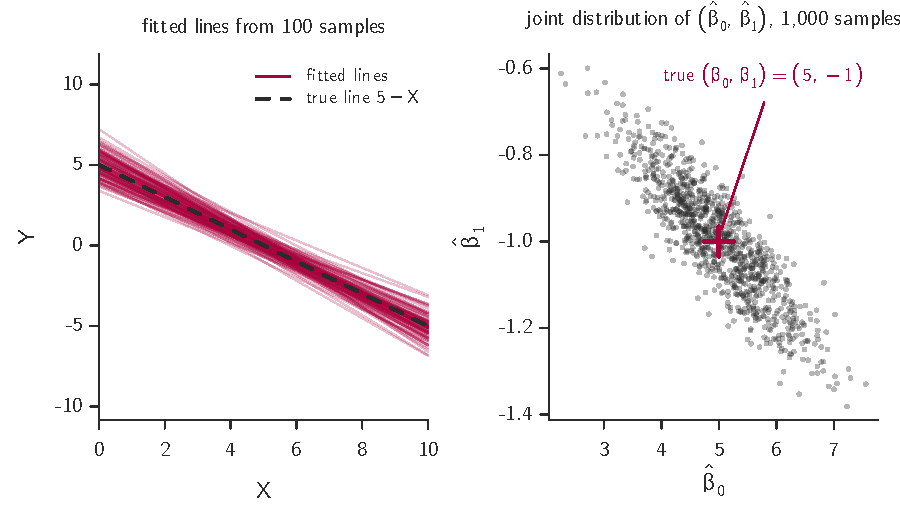
\includegraphics[height=0.82\textheight]{sim_lines_joint.pdf}
\end{figure}

}

\frame{
\frametitle{Sampling Distribution of $\hat{\beta}_0$ and $\hat{\beta}_1$}
\vspace{-.3cm}
\begin{figure}[ht] \centering
        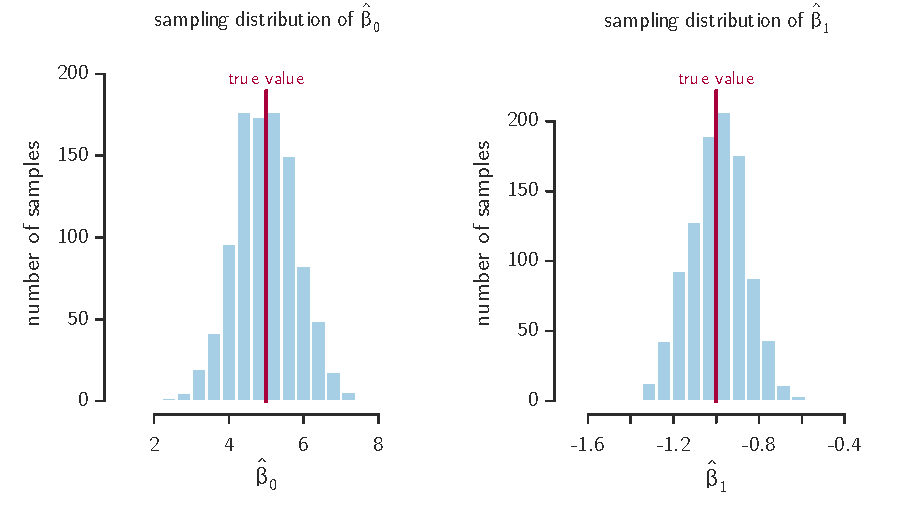
\includegraphics[height=0.82\textheight]{sim_marginals.pdf}
\end{figure}

}

\subsection{Unbiasedness of OLS Estimators}

\frame{
\frametitle{Unbiasedness of OLS}
\begin{theorem}[Unbiasedness of OLS]
Given OLS Assumptions I--IV:
$$
E[\hat{\beta}_0] \ = \ \beta_0 \quad \text{ and } \quad E[\hat{\beta}_1] \ = \ \beta_1
$$
The sampling distributions of the estimators $\hat{\beta}_1$ and $\hat{\beta}_0$ are centered about the true population parameter values $\beta_1$ and $\beta_0$.
\end{theorem}\bigskip

\textbf{Worksheet Q1}: Prove: $E[\hat{\beta}_1] \ = \ \beta_1$.\\ \bigskip

%\begin{block}{Proof} \pause
  % $\hat{\beta}_1 = \frac{\sum_{i=1}^n (x_i - \bar{x})(y_i -
%   \bar{y})}{\sum_{i=1}^n(x_i - \bar{x})^2}=\pause \frac{\sum_{i=1}^n (x_i - \bar{x})y_i}{SST_x}$
% {\scriptsize (Note: $\sum_{i=1}^n(x_i - \bar{x})\bar{y} = 0$)}  \\\medskip \pause
% $\quad =   \frac{\sum_{i=1}^n (x_i - \bar{x})(\beta_0+\beta_1 x_i + u_i)}{SST_x} =  \pause \frac{\beta_0 \sum_{i=1}^n (x_i - \bar{x})+ \beta_1 \sum_{i=1}^n (x_i - \bar{x})x_i + \sum_{i=1}^n (x_i - \bar{x})u_i}{SST_x} $\\\medskip \pause
% $\quad =  \frac{\beta_0 \cdot 0 + \beta_1 \sum_{i=1}^n (x_i - \bar{x})^2 + \sum_{i=1}^n (x_i - \bar{x})u_i}{SST_x}$  \\\medskip \pause
% $\quad =  \frac{\beta_1 SST_x + \sum_{i=1}^n (x_i - \bar{x})u_i}{SST_x} = \pause  \beta_1 + \frac{\sum_{i=1}^n (x_i - \bar{x})u_i}{SST_x}$ {\scriptsize (continued...)}
%\end{block}
Proof for the intercept is analogous.
}



% \frame{
% \frametitle{Unbiasedness of OLS}
% \begin{proof}[Proof (Cont.)]
% Therefore,
% \begin{eqnarray*}
% E[\hat{\beta}_1\mid X] & = & E[\beta_1\mid X] + E\l[\frac{\sum_{i=1}^n(x_i-\bar{x})u_i}{SST_x} \big| X\r] \\
% & = & \beta_1 + \sum_{i=1}^n \frac{(x_i-\bar{x})}{SST_x} E[u_i\mid X] \\ \pause
% & = & \beta_1 \quad \text{(the zero conditional mean assumption)}
% \end{eqnarray*}
% \pause
% Finally, by the law of iterated expectations,
% $$ E[\hat{\beta}_1] \ = \ E[E[\hat{\beta}_1\mid X]] \ = \ \beta_1. $$
% \end{proof}
% \pause
% Proof for the intercept is analogous.
% }

\frame{
\frametitle{Example: Binary Independent Variable}
\small
Suppose \alert{Assumptions I--IV} hold for a simple regression model with $X=0$ or $X=1$,
which may be the indicator of an experimental treatment.
$$
Y = \beta_0 + \beta_1 X + u
$$

In this case, the OLS slope estimator $\hat{\beta}_1$ from the regression of $Y$ on $X$ is unbiased for $\beta_1$, the expected effect of the treatment on $Y$. \pause
\begin{align*}
E[Y|X=1] &= \beta_0 + \beta_1 E[X|X=1] + E[u|X=1] \\
&= \beta_0 + \beta_1
\end{align*} \pause
\begin{align*}
E[Y|X=0] &= \beta_0 + \beta_1 E[X|X=0] + E[u|X=0] \\
&= \beta_0
\end{align*} \pause
$$
E[Y|X=1] -E[Y|X=0] = \beta_1
$$
}

\frame{

\frametitle{Example: Binary Independent Variable}
\small
Suppose we drop Assumption IV ($E[u|X]=0$) and so only
\alert{Assumptions I--III} hold for our regression model with $X=0$ or $X=1$.
$$
Y = \beta_0 + \beta_1 X + u
$$
In this case, the OLS slope estimator $\hat{\beta}_1$ from the regression of $Y$ on $X$ is generally biased for $\beta_1$, the expected effect of the treatment on $Y$. \pause
\begin{align*}
E[Y|X=1] &= \beta_0 + \beta_1 E[X|X=1] + E[u|X=1] \\
&= \beta_0 + \beta_1  + E[u|X=1]
\end{align*} \pause
\begin{align*}
E[Y|X=0] &= \beta_0 + \beta_1 E[X|X=0] + E[u|X=0] \\
&= \beta_0  + E[u|X=0]
\end{align*}\pause
\begin{equation}
E[Y|X=1] -E[Y|X=0]=\underbrace{\beta_1}_{\mbox{Effect}}
                 +\underbrace{\{E[u|X=1] - E[u|X=0]\}}_{\mbox{BIAS}}\nonumber
\end{equation}
}

\frame{
\frametitle{Example: Telling People How Many Immigrants There Are}
\small
\begin{columns}[T]
\begin{column}{0.55\textwidth}
\begin{itemize}
\item An online survey in March 2017. A random draw put each respondent in a group.
\item $X=1$: told that the Census Bureau estimates about 13 of every 100 people in the U.S.\ were born abroad.\\
  $X=0$: told nothing.
\item Then everyone answered three questions about immigration and guessed again how many of every 100 people in the U.S.\ were born abroad.
\pause
\medskip
\item A random draw set $X$, so the two groups are alike on average in everything else, and $E[u|X=1]=E[u|X=0]$.
\item[] $\longrightarrow$ \alert{Assumption IV holds by design}, and the bias term on the last slide is zero.
\end{itemize}
\end{column}
\begin{column}{0.43\textwidth}
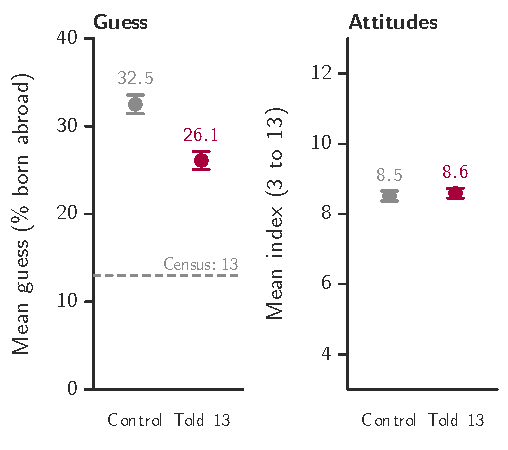
\includegraphics[width=\linewidth]{hopkins_means.pdf}\\
{\scriptsize Group means with 95\% intervals. The attitude index adds up the three answers, 3 to 13 (higher = more restrictive).}
\end{column}
\end{columns}
\slidesource{Hopkins, Sides \& Citrin (2019), \emph{Journal of Politics} 81(1); their 2017 Morning Consult survey (non-Hispanic respondents; control vs.\ information groups).}
}

\begin{frame}[fragile]
\frametitle{Binary $X$ in R: The Slope Is a Difference in Means}
{\spacingset{0.8}
\footnotesize
\begin{Verbatim}[frame=single, label=R Code, commandchars=\\\{\}]
> lm.guess <- lm(guess ~ info, data = hsc)
> summary(lm.guess)

~~~~ output omitted ~~~~

Coefficients:
            Estimate Std. Error t value Pr(>|t|)
(Intercept)  \textcolor{red}{32.4943}     0.5258  61.796   <2e-16 ***
info         \textcolor{red}{-6.3941}     0.7484  -8.544   <2e-16 ***

Residual standard error: 23.09 on 3806 degrees of freedom
\end{Verbatim}
}
\small
\begin{itemize}
\item $\hat\beta_0 = 32.5$ is the mean guess when $X=0$, and $\hat\beta_0+\hat\beta_1 = 26.1$ is the mean guess when $X=1$. So $\hat\beta_1 = -6.39$ (SE~0.75, $t=-8.54$, $N=3{,}808$) is the difference in means.
\pause
\item The guesses are skewed. The median falls from 25 to 13, but the mean only from 32.5 to 26.1.
\pause
\item Attitudes barely move. The same regression with the attitude index gives $\hat\beta_1 = +0.08$ ($t=0.77$).
\end{itemize}
\end{frame}



\subsection{Variance of OLS Estimators}

\frame{

\frametitle{Variance of OLS Estimators}
\small
\begin{itemize}
\item Given unbiasedness we now know the means of the sampling distributions of our estimators $\hat{\beta}_1$ and $\hat{\beta}_0$.
\item What about the variances of the sampling distributions, $\var[\hat{\beta}_0]$ and $\var[\hat{\beta}_1]$?
\end{itemize}

\begin{figure}[ht] \centering
        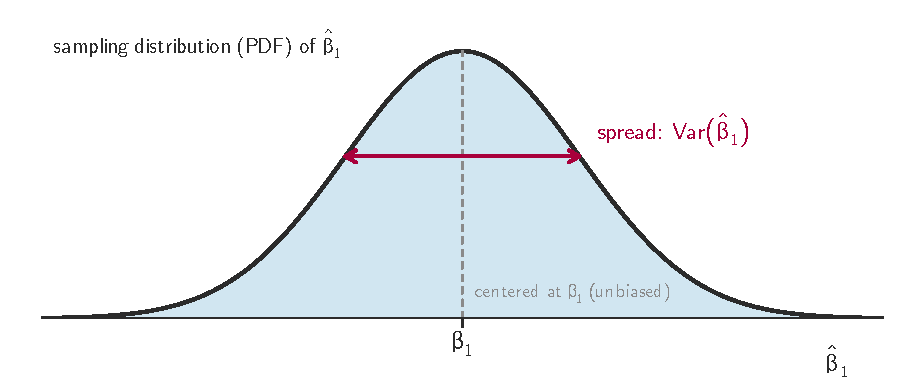
\includegraphics[height=0.66\textheight]{var_beta1.pdf}
\end{figure}

}


\frame{

\frametitle{Variance of OLS Estimators}
\small
How can we derive $\var[\hat{\beta}_0]$ and $\var[\hat{\beta}_1]$? Let's make the
following additional assumption:\pause
\begin{assumption}[V. Homoskedasticity]
The conditional variance of the error term is constant and does not vary as a function
of the explanatory variable:
$$ \var[u|X]=\sigma^2_u $$
\end{assumption}
\pause
\begin{itemize}
\item This implies $\var[u] = \sigma^2_u$ \\
 $\rightarrow$ all errors have an identical \alert{error variance}
($\sigma^2_{u_i}=\sigma^2_u$ for all $i$) \pause
 \item Taken together, Assumptions I--V imply:
$$
E[Y|X] \ = \ \beta_0 + \beta_1 X  $$
$$
\var[Y|X] \ = \ \sigma^2_u
$$
\pause
\vspace{-\baselineskip}
\item Violation: $\var[u|X=x_1] \neq \var[u|X=x_2]$ called \alert{heteroskedasticity}.
\item Assumptions I--V are collectively known as the \alert{Gauss-Markov assumptions}
\end{itemize}
}

\frame{
\frametitle{Homoskedasticity}

\vspace{-.3cm}
\begin{figure}[ht] \centering
        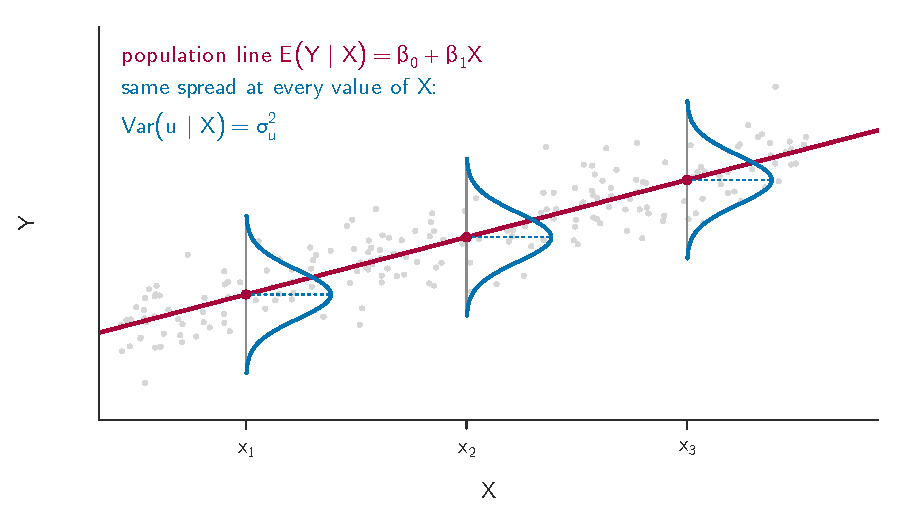
\includegraphics[height=0.82\textheight]{cond_homo.pdf}
\end{figure}

}

\frame{
\frametitle{Heteroskedasticity}

\vspace{-.3cm}
\begin{figure}[ht] \centering
        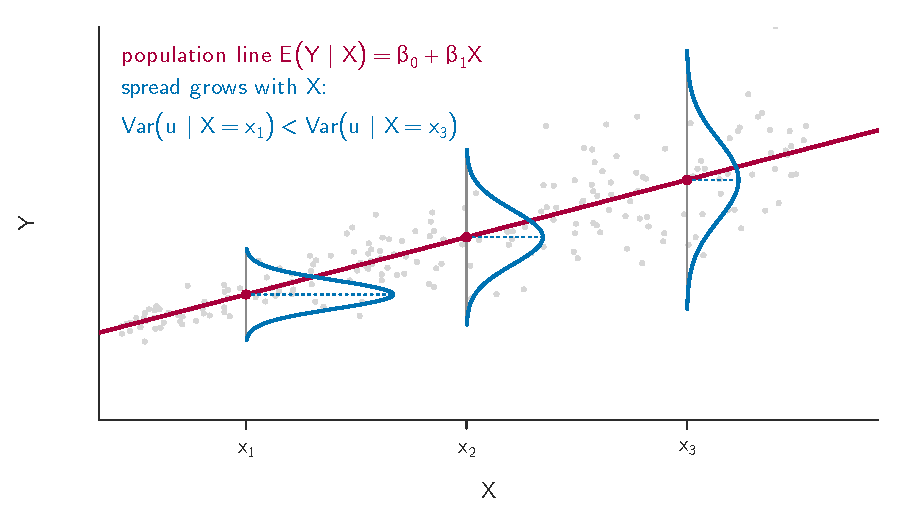
\includegraphics[height=0.82\textheight]{cond_hetero.pdf}
\end{figure}

}

\frame[t]{
\frametitle{Variance of OLS Estimators}
\small
\begin{theorem}[Variance of OLS Estimators]
Given OLS Assumptions I--V (Gauss-Markov Assumptions):
$$
\var[\hat{\beta}_1\mid X]=\frac{\sigma^2_u}{\sum_{i=1}^n (x_i - \bar{x})^2}=\frac{\sigma^2_u}{SST_x}
$$
$$
\var[\hat{\beta}_0\mid X]=\sigma^2_u \left\{\frac{1}{n} +\frac{\bar{x}^2}{\sum_{i=1}^n (x_i-\bar{x})^2}\right\}
$$
where $\var[u\mid X]=\sigma^2_u$ (the error variance).
\end{theorem}

\bigskip\textbf{Worksheet Q2}: Show $\var[\hat{\beta}_1\mid X]=\frac{\sigma^2_u}{\sum_{i=1}^n (x_i - \bar{x})^2}$
}

% \frame[t]{
% \frametitle{Variance of OLS Estimators}
% \small
% \begin{theorem}[Variance of OLS Slope Estimator]
% Given OLS Assumptions I--V (Gauss-Markov Assumptions):
% $$
% \var[\hat{\beta}_1\mid X]=\frac{\sigma^2_u}{\sum_{i=1}^n (x_i - \bar{x})^2}=\frac{\sigma^2_u}{SST_x}
% $$
% \end{theorem}
% \vspace{-.075in}
% \begin{proof}
% \vspace{-.125in}
% {\scriptsize
% \begin{eqnarray*}
% \hat{\beta}_1 & = & \beta_1 + \frac{\sum_{i=1}^n (x_i - \bar{x})}{SST_x}u_i \pause \\
% V\l[\hat{\beta}_1\mid X \r] & = &
%    V\l[\beta_1\mid X\r] + V\l[\sum_{i=1}^n \frac{(x_i - \bar{x})u_i}{SST_x} \Big| X\r] \pause \\
% & = & \sum_{i=1}^n \left\{\frac{(x_i - \bar{x})}{SST_x}\right\}^2 \var[u_i\mid X] \\ \pause
% & = & \frac{\sum_{i=1}^n(x_i - \bar{x})^2}{SST_x^2} \sigma^2_u
% \ = \ \frac{SST_x}{SST^2_x}\sigma^2_u \ = \ \frac{\sigma^2_u}{SST_x}.
% \end{eqnarray*}
% The proof for $\hat\beta_0$ is analogous.
% }
% \end{proof}
% }


\begin{frame}[t]
\frametitle{Intuition for the Variance of Slope Estimator}
$$
\var[\hat{\beta}_1\mid X]=\frac{\sigma^2_u}{\sum_{i=1}^n (x_i - \bar{x})^2}
$$
Do we know $\sigma^2_u$? \pause \ No. \pause

But let's assume we do for now and ask: What factors affect $\var[\hat{\beta}_1\mid X]$?\\\medskip
Variance is low if \pause
\begin{enumerate}
  \item Error variance $\var[u]=\sigma^2_u$ is low.
\end{enumerate}

\end{frame}

\frame{
\frametitle{Error Variance and $\var[\hat{\beta}_1]$}
\scriptsize
\vspace{-.3cm}
\begin{figure}[ht] \centering
        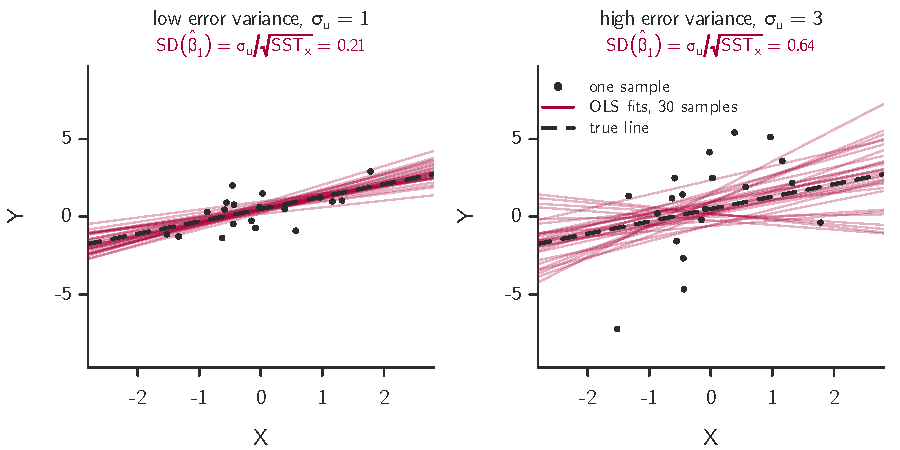
\includegraphics[height=0.74\textheight]{var_sigma.pdf}
\end{figure}
Approximation of true slope is better if $\var[u]=\sigma^2_u$ is lower (for fixed $x$, $\beta_1$, $\beta_0$)
}

\begin{frame}
\frametitle{Intuition for Variance of Slope Estimator}
$$
\var[\hat{\beta}_1\mid X]=\frac{\sigma^2_u}{\sum_{i=1}^n (x_i - \bar{x})^2}
$$
\invisible{
Do we know $\sigma^2_u$? \ No.

But let's assume we did and ask: What factors determine $\var[\hat{\beta}_1\mid X]$?\\\medskip
}
Variance is low if
\begin{enumerate}
  \item Error variance $\var[u]=\sigma^2_u$ is low.\medskip\pause
  \item Note that
  $$\sum_{i=1}^n (x_i - \bar{x})^2 = (n-1) S_x^2 $$
  where $S_x^2$ is the sample variance of $X$. Therefore,
  \begin{itemize}\medskip
    \item $\var[\hat{\beta}_1\mid X]$ decreasing in $n$ (holding $S_x^2$ fixed)\medskip
    \item $\var[\hat{\beta}_1\mid X]$ decreasing in $S_x^2$ (holding $n$ fixed)
  \end{itemize}
\end{enumerate}
%Recall that for testing and to construct CIs we will need the standard deviation of the sampling distribution. This is called the \alert{standard error}:
%$SD(\hat{\beta}_1)=\sigma/\sqrt{SST_x}$
\end{frame}

\frame{
\frametitle{$\var[x]$ and $\var[\hat{\beta}_1]$}
\scriptsize
\vspace{-.3cm}
\begin{figure}[ht] \centering
        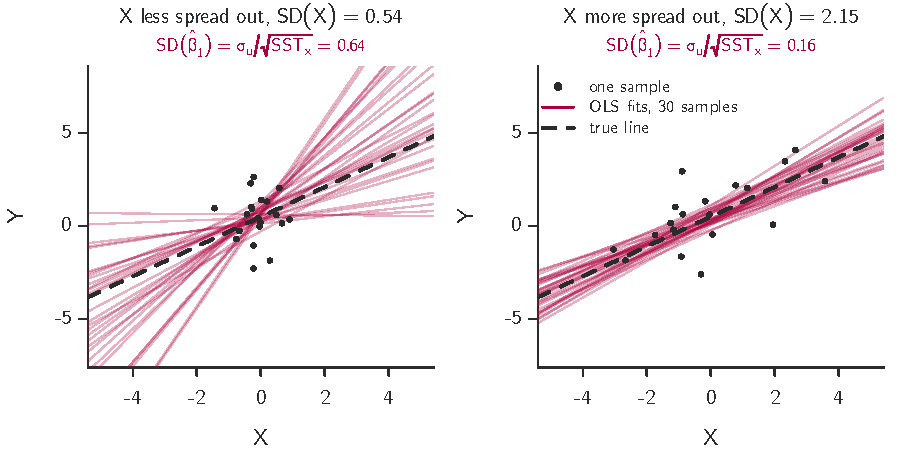
\includegraphics[height=0.74\textheight]{var_spreadx.pdf}
\end{figure}
Approximation of true slope is better if $\var[x]$ is higher (for fixed $\sigma_u$, $\beta_1$, $\beta_0$)
}


\subsection{Estimating Variance for Slope and Intercept}

\frame{
\frametitle{Estimating the Variance of OLS Estimators}
\small
How can we estimate the unobserved error variance $Var[u]=\sigma^2_u$? \\
\pause We can derive an estimator based on the \alert{residuals}:
$$
\hat{u}_i \ = \ y_i - \hat{y}_i \ = \ y_i - \hat{\beta}_0 - \hat{\beta}_1 x_i
$$
Recall: The \alert{errors} $u_i$ are NOT the same as the residuals $\hat{u}_i$.\\\medskip
\pause
Intuitively, the scatter of the residuals around the fitted regression line should reflect the unseen scatter about the true population regression line.\\\medskip

We can measure scatter with the mean squared deviation:
$$ MSD(\hat{u})\equiv\frac{1}{n}\sum_{i=1}^n (\hat{u}_i-\bar{\hat{u}})^2=\pause\frac{1}{n}\sum_{i=1}^n \hat{u}_i^2$$
\pause
Intuitively, which line is likely to be closer to the observed sample values on $X$ and $Y$, the true line $E[Y\mid X=x_i] = \beta_0 + \beta_1 x_i$ or the fitted regression line $\hat{y}_i = \hat{\beta}_0 + \hat{\beta}_1 x_i$?

}

\frame{
\frametitle{Estimating the Variance of OLS Estimators}
\small
\begin{itemize}
\item By construction, the regression line is closer since it is drawn to fit the actual sample we have
\pause
\item Specifically, the regression line is drawn so as to minimize the sum of the squares of the distances between it and the observations

\pause
\medskip

\item So the spread of the residuals $MSD(\hat{u})$ will slightly {\it underestimate} the error variance $\var[u]=\sigma^2_u$ on average
\pause
\item In fact, we can show that with a single regressor $X$ we have:
$$
E[MSD(\hat{u})]=\frac{n-2}{n}\sigma^2_u \mbox{ (degrees of freedom adjustment)}
$$
\pause
\item Thus, an \alert{unbiased estimator} for the error variance is:
$$
\hat{\sigma}^2_u = \frac{n}{n-2} MSD(\hat{u}) = \frac{n}{n-2} \frac{1}{n}\sum_{i=1}^n \hat{u}_i^2 = \frac{1}{n-2}\sum_{i=1}^n \hat{u}^2_i
$$
We plug this estimate into the variance estimators for $\hat{\beta}_0$ and $\hat{\beta}_1$.
\end{itemize}
}


\frame{
\frametitle{Estimating the Variance of OLS Estimators}

Given Assumptions I--V (Gauss-Markov Assumptions), we can then estimate the variance of the slope and intercept as:
$$
\widehat{V}[\hat{\beta}_1\mid X]=\frac{\hat{\sigma}^2_u}{\sum_{i=1}^n (x_i - \bar{x})^2}
$$
$$
\widehat{V}[\hat{\beta}_0\mid X]=\hat{\sigma}^2_u \left\{\frac{1}{n} +\frac{\bar{x}^2}{\sum_{i=1}^n (x_i-\bar{x})^2}\right\}
$$
where $\hat{\sigma}^2_u = \frac{1}{n-2}\sum_{i=1}^n \hat{u}^2_i$\\\bigskip

The estimated standard errors of the slope and the intercept are $\sqrt{\widehat{V}[\hat{\beta}_1\mid X]}$ and $\sqrt{\widehat{V}[\hat{\beta}_0\mid X]}$, respectively.
}

\begin{frame}[fragile]
\frametitle{College Degrees and the 2024 Trump Vote, 50 States}
{\spacingset{0.8}
\footnotesize
\begin{Verbatim}[frame=single, label=R Code, commandchars=\\\{\}]
> lm.out <- lm(trump ~ ba, data = states)
> summary(lm.out)

~~~~ output omitted ~~~~

Coefficients:
            Estimate Std. Error t value Pr(>|t|)
(Intercept) \textcolor{red}{102.8376}     \textcolor{red}{5.9818}  17.192  < 2e-16 ***
ba           \textcolor{red}{-1.4537}     \textcolor{red}{0.1738}  -8.366  6.2e-11 ***
---
Signif. codes:  0 '***' 0.001 '**' 0.01 '*' 0.05 '.' 0.1 ' ' 1

Residual standard error: 6.589 on 48 degrees of freedom
Multiple R-squared:  \textcolor{red}{0.5932},	Adjusted R-squared:  0.5847
F-statistic: 69.99 on 1 and 48 DF,  p-value: 6.199e-11
\end{Verbatim}
}
\small
\begin{itemize}
\item By hand, $\hat\sigma^2_u = \sum_i \hat u_i^2/(n-2) = 2{,}083.9/48 = 43.4$. With $\sum_i (x_i-\bar x)^2 = 1{,}437.9$, the standard error of $\hat\beta_1$ is $\sqrt{43.4/1{,}437.9} = 0.174$.
\item Assumption II is a model here. The 50 states are the whole population of states. We treat each state's vote as one draw of $Y$ given its $X$.
\item Assumption V looks reasonable. The residuals spread about equally across $X$ (a Breusch--Pagan test, taught in Lecture 6-3, gives $p = .75$).
\end{itemize}
\end{frame}

\subsection{Gauss-Markov Theorem}

\frame{
\frametitle{Gauss-Markov Theorem}
\begin{theorem}[Gauss-Markov]
Given OLS Assumptions I--V, the OLS estimator is \alert{BLUE}, i.e. the
\begin{enumerate}
  \item \alert{B}est: Lowest variance in class
  \item \alert{L}inear: Among Linear estimators
  \item \alert{U}nbiased: Among Linear Unbiased estimators
  \item \alert{E}stimator.
\end{enumerate}
\end{theorem}
\begin{proof}
This proof is not terribly insightful and low priority so we take it on trust \\
(read up on it in Wooldridge, \emph{Introductory Econometrics}, 3rd ed., Appendix 3A.6!).
\end{proof}
}


\frame{
\frametitle{Gauss-Markov Theorem}
% Redrawn in TikZ (2026-09-17) from BLUE.pdf, a scanned 1999 tutorial page.
\begin{center}
\begin{tikzpicture}[x=1pt,y=1pt]
  \draw[CourseInk, line width=0.6pt] (-165,-92) rectangle (165,92);
  \node[anchor=north west, font=\small] at (-161,88) {All estimators};
  \begin{scope}
    \clip (0,0) ellipse (40 and 80);
    \fill[Cardinal!15] (0,0) ellipse (110 and 36);
  \end{scope}
  \draw[CourseBlue, line width=1pt] (0,0) ellipse (40 and 80);
  \draw[Cardinal, line width=1pt] (0,0) ellipse (110 and 36);
  \node[CourseBlue, font=\small, anchor=west] (ub) at (60,72) {unbiased};
  \draw[CourseBlue, -{Latex[length=4pt]}] (ub.west) to[bend right=15] (30,53);
  \node[Cardinal, font=\small, anchor=west] (li) at (115,46) {linear};
  \draw[Cardinal, -{Latex[length=4pt]}] (li.west) to[bend right=15] (92,20);
  \fill[Cardinal] (-8,-4) circle (2.4pt);
  \node[font=\scriptsize, anchor=west, text=CourseInk] at (-5,-4) {OLS};
  \node[font=\scriptsize, align=center, text=CourseInk] at (-86,-62)
    {shaded: linear \emph{and} unbiased};
  \draw[CourseInk, -{Latex[length=4pt]}] (-80,-55) to[bend left=10] (-24,-14);
  \node[font=\scriptsize, align=center, text=CourseInk] at (92,-62)
    {OLS has the lowest variance\\in the shaded class (BLUE)};
\end{tikzpicture}
\end{center}

}

\end{document}
